%%%%%%%%%%%%%%%%%%%%%%%%%%%%%%%%%%%%%%%%%
% University Assignment Title Page 
% LaTeX Template
% Version 1.0 (27/12/12)
%
% This template has been downloaded from:
% http://www.LaTeXTemplates.com
%
% Original author:
% WikiBooks (http://en.wikibooks.org/wiki/LaTeX/Title_Creation)
%
% License:
% CC BY-NC-SA 3.0 (http://creativecommons.org/licenses/by-nc-sa/3.0/)
% 
% Instructions for using this template:
% This title page is capable of being compiled as is. This is not useful for 
% including it in another document. To do this, we have two options: 
%
% 1) Copy/paste everything between \begin{document} and \end{document} 
% starting at \begin{titlepage} and paste this into another LaTeX file where we 
% want your title page.
% OR
% 2) Remove everything outside the \begin{titlepage} and \end{titlepage} and 
% move this file to the same directory as the LaTeX file we wish to add it to. 
% Then add \input{./title_page_1.tex} to your LaTeX file where we want your
% title page.
%
%%%%%%%%%%%%%%%%%%%%%%%%%%%%%%%%%%%%%%%%%
%\title{Title page with logo}
%----------------------------------------------------------------------------------------
%	PACKAGES AND OTHER DOCUMENT CONFIGURATIONS
%----------------------------------------------------------------------------------------

\documentclass[11pt]{article}
\usepackage[italian]{babel}
\usepackage[utf8x]{inputenc}
\usepackage{amsmath}
\usepackage{graphicx}
\usepackage[colorinlistoftodos]{todonotes}
\usepackage{enumitem}
\usepackage{listings}
\usepackage{filecontents}
\usepackage{verbatim}
\usepackage{eurosym}
\usepackage[export]{adjustbox}

\usepackage{float}
\usepackage[margin=3cm]{geometry}
\usepackage{listings}
\usepackage{xcolor}

\definecolor{codegreen}{rgb}{0,0.6,0}
\definecolor{codegray}{rgb}{0.5,0.5,0.5}
\definecolor{codepurple}{rgb}{0.58,0,0.82}
% \definecolor{backcolour}{rgb}{0.95,0.95,0.95}
\definecolor{backcolour}{rgb}{1,1,1}

\lstdefinestyle{mystyle}{
    backgroundcolor=\color{backcolour},   
    commentstyle=\color{codegreen},
    keywordstyle=\color{magenta},
    numberstyle=\tiny\color{codegray},
    stringstyle=\color{codepurple},
    basicstyle=\ttfamily\footnotesize,
    aboveskip=15pt, % Adjust the space above the listing
    belowskip=15pt, % Adjust the space below the listing
    breakatwhitespace=false,         
    breaklines=true,                 
    captionpos=b,                    
    keepspaces=true,                 
    numbers=left,                    
    numbersep=5pt,                  
    showspaces=false,                
    showstringspaces=false,
    showtabs=false,                  
    tabsize=2
}

\lstset{style=mystyle}

\begin{document}
\begin{titlepage}

    \newcommand{\HRule}{\rule{\linewidth}{0.5mm}} % Defines a new command for the horizontal lines, change thickness here

    \center % Center everything on the page

    %----------------------------------------------------------------------------------------
    %	HEADING SECTIONS
    %----------------------------------------------------------------------------------------

    \textsc{\LARGE Università di Messina}\\[1.5cm] % Name of your university/college
    \textsc{\Large Dipartimento di scienze matematiche e informatiche, scienze fisiche e della terra}\\[0.5cm] % Major heading such as course name
    \textsc{\large Corso di Laurea Triennale in Informatica}\\[0.5cm] % Minor heading such as course title

    %----------------------------------------------------------------------------------------
    %	TITLE SECTION
    %----------------------------------------------------------------------------------------

    \HRule \\[0.4cm]
    { \huge \bfseries Distributed computation of linear algebra operations}\\[0.4cm] % Title of your document
    \HRule \\[1.5cm]

    %----------------------------------------------------------------------------------------
    %	AUTHOR SECTION
    %----------------------------------------------------------------------------------------

    \begin{minipage}{0.4\textwidth}
        \begin{flushleft} \large
            \emph{Author:}\\
            Gabriele \textsc{Aloisio} \textit{(503264)} \\
        \end{flushleft}
    \end{minipage}
    ~
    \begin{minipage}{0.4\textwidth}
        \begin{flushright} \large
            \emph{Supervisor:} \\
            prof. Roberto \textsc{Marino} \\
        \end{flushright}
    \end{minipage}\\[2cm]

    % If we don't want a supervisor, uncomment the two lines below and remove the section above
    %\Large \emph{Author:}\\
    %John \textsc{Smith}\\[3cm] % your name

    %----------------------------------------------------------------------------------------
    %	DATE SECTION
    %----------------------------------------------------------------------------------------

    {\large \today}\\[2cm] % Date, change the \today to a set date if we want to be precise

    %----------------------------------------------------------------------------------------
    %	LOGO SECTION
    %----------------------------------------------------------------------------------------

    
\includegraphics[width=70px, keepaspectratio]{unime.png}\\[1cm] % Include a department/university logo - this will require the graphicx package

    %----------------------------------------------------------------------------------------

    \vfill % Fill the rest of the page with whitespace

\end{titlepage}

\tableofcontents
\pagebreak

\section{Abstract}
Our study explores the performance of distributed linear algebra operations executed in both serial and parallel modes across varying matrix sizes. We find that serial execution outperforms parallel execution, especially for smaller matrices, but as matrix size increases, the performance gap widens. This suggests that parallelization's overhead can outweigh its advantages for larger matrices. Additionally, standard deviation in execution times increases with matrix size. Our case study uses the Ray framework on a 10-computer cluster provided by the University of Messina. The cluster performs our tests of determinant, dot product, matrix inversion, and rank calculations across different matrix sizes.

\section{Introduction}
Matrix operations are fundamental in numerous scientific and computational domains, serving as the building blocks for various applications. However, traditional sequential computation on a single machine often becomes a bottleneck, limiting the speed and scalability of matrix calculations. To address this problem, we are going to use an open-source distributed computing framework called \textbf{Ray}.

\subsection{Overview of distributed systems and networks}
A distributed system consists of multiple interconnected computers that collaborate and coordinate their activities to achieve a common goal. These systems are designed to tackle tasks that cannot be efficiently computed by a single machine. Networks serve as the backbone of distributed systems, enabling communication among the connected nodes. Network infrastructures enable coordination, data sharing, and synchronization across distributed systems, regardless of their physical locations.

\subsection{The Ray library}
The Ray library is an open-source distributed computing framework primarily designed for building scalable and high-performance applications. It was developed by the company Anyscale, which aimed to simplify the development of distributed and parallel computing applications. When it comes to matrix operation computation, using Ray for distributed computation offers several advantages over performing the operations on a single machine:
\begin{itemize}
    \item \textbf{Faster execution}: With Ray we can use multiple machines and CPUs to compute operations. This significantly reduces the computation time compared to a single machine. Each machine can work on a subset of the matrix data, completing the calculations in parallel. This distributed approach can lead to substantial speedups.
    \item \textbf{Scalability}: As the size of the matrices grows, a single machine may struggle to handle the computational demands due to memory limitations or processing power constraints. Ray allows we to scale horizontally by adding more machines to the distributed setup.
    \item \textbf{Fault tolerance}: Ray offers fault tolerance mechanisms that ensure the continuity of computation even in the presence of failures. If a machine participating in the distributed computation fails, Ray can automatically redistribute the workload to other available machines.
    \item \textbf{Resource utilization}: With Ray, each machine contributes its processing power and memory capacity to the overall computation. This efficient utilization of resources allows we to make the most of the available hardware infrastructure, compared to a single machine that may be underutilized.
\end{itemize}

\subsection{Python}
Python is a versatile and high-level programming language known for its simplicity and readability. It is widely used for a variety of applications, including web development, data analysis, artificial intelligence, scientific computing, and automation. Python's strength lies in its support for multiple programming paradigms, including procedural, object-oriented, and functional programming. Its large and active community contributes to a vast ecosystem of libraries and frameworks, making it a powerful tool for a wide range of tasks.
\\\\
In the context of this paper, Python serves as the primary programming language for conducting tests and implementing linear algebra operations. Additionally, Matplotlib is utilized for graphing and visualizing the results of these tests.
\\\\
The object-oriented programming (OOP) paradigm has been employed in this research to represent matrices. This approach enhances code organization and readability while facilitating the implementation of complex linear algebra operations.
\\\\
It's worth noting that Python is one of the two languages supported by Ray, with the other being Java, making it a suitable choice for distributed computing and parallelization.

\section{Case study}

In this section, we present the case study conducted to evaluate the performance of distributed computation of linear algebra operations using Ray 2.4.0 on a cluster comprised of 10 computers with specifications provided by the University of Messina. The experiments include the caluclation of determinant, dot product, matrix inversion, and rank. For both serial and parallel execution, we conducted tests with increasing matrix sizes and repetitions to gather comprehensive performance data.
\\\\
The cluster used for our experiments is composed of ten computers with the following specifications, provided by the University of Messina:
\begin{itemize}
    \item {RAM: 8GB}
    \item {CPU: DA INSERIRE}
\end{itemize}
\pagebreak
\subsection{Execution of tests}
For our experiments, we considered the following parameters:
\begin{itemize}
    \item \textbf{Determinant calculation:} Matrices of sizes $n = 2 \dots 10$ were used, with each $n$ value being executed three times. The average execution time was recorded for analysis.
    \item \textbf{Dot product:} Matrices of sizes $n = 2 \dots 30$ were employed, with each $n$ value being executed five times.
    \item \textbf{Inverse:} Matrices of sizes $n = 2 \dots 8$ were utilized, with each $n$ value being executed three times.
    \item \textbf{Rank:} Matrices of sizes $n = 2 \dots 500$ were tested, with each $n$ value being executed five times.
\end{itemize}
\vfill
For each type of operation, the code iterates through different matrix sizes, executing the operation multiple times for each size to capture variations in performance, and recording the execution times for analysis. The results of these tests are stored in separate CSV files, organized by operation type and parameter configuration. This is achieved with the following Python script:
\pagebreak
\begin{lstlisting}[language=Python, label=main.py]
import ray
from matrix_serial import Matrix
import time
import csv
    
def test_dot(l, u, runs, filename):
    '''Make tests for matrices size l...u'''
    max_n = (u-l)*runs
    counter = 0
    measures = []
    
    print(f"running test_dot with l={l}, u={u}, runs={runs}")

    for n in range(l, u):
        sub_run = []
        sub_run.append(n) # matrix size

        for i in range(runs):
            a = Matrix.random_int(n, n, -10**8, 10**8)
            b = Matrix.random_float(n, n, -99, 99)

            t0 = time.time()
            Matrix.dot(a,b)
            t1 = time.time()

            sub_run.append(t1-t0)

            counter += 1
            print(f"run # {counter}/{max_n}: {t1-t0}")

        measures.append(sub_run)

    with open(f"{filename}_{l}_{u}_{runs}.csv", "w") as f:
        writer = csv.writer(f)
        writer.writerows(measures)

    return measures

def test_det(l, u, runs, filename):
    [...]
def test_rank(l, u, runs, filename):
    [...]
def test_inv(l, u, runs, filename):
    [...]

if __name__ == "__main__":
    if ray.is_initialized:
        ray.shutdown()
    ray.init(include_dashboard=True)

    test_det(2, 10, 3, "test_results/[[serial/parallel]]/det")
    test_dot(2, 30, 5, "test_results/[[serial/parallel]]/dot")
    test_inv(2, 8, 3, "test_results/[[serial/parallel]]/inv")
    test_rank(2, 500, 5, "test_results/[[serial/parallel]]/rank")
    \end{lstlisting}

\subsection{Graphing the results}
The code loads CSV files onto defined variables and then generates plots with error bars to visualize the performance differences between serial and parallel execution using \textit{matplotlib}. The primary goal is to assess the efficiency and scalability of these operations when executed in parallel. The resulting plots are saved as PNG files for analysis.
\\\\
A different function was defined for the plotting of rank, downsampling the data. This is because of its particular case of increasing standard deviation value, thus legibility reasons.

\begin{lstlisting}[language=Python, label=plots.py]
import csv
import matplotlib.pyplot as plt
import numpy as np

def serial_parallel_comparison(csv_name, func_name):
    # Read data from serial CSV file
    serial_data = []
    with open(f"test_results/serial/{csv_name}", "r") as f:
        reader = csv.reader(f)
        for row in reader:
            serial_data.append([float(val) for val in row])

    # Read data from parallel CSV file
    parallel_data = []
    with open(f"test_results/parallel/{csv_name}", "r") as f:
        reader = csv.reader(f)
        for row in reader:
            parallel_data.append([float(val) for val in row])

    # Extract serial data
    serial_sizes = [run[0] for run in serial_data]
    serial_means = [np.mean(runs) for runs in serial_data]
    serial_std_devs = [np.std(runs) for runs in serial_data]

    # Extract parallel data
    parallel_sizes = [run[0] for run in parallel_data]
    parallel_means = [np.mean(runs) for runs in parallel_data]
    parallel_std_devs = [np.std(runs) for runs in parallel_data]

    # Plot data
    plt.errorbar(serial_sizes, serial_means, yerr=serial_std_devs, fmt='o-', label='Serial Execution Time')
    plt.errorbar(parallel_sizes, parallel_means, yerr=parallel_std_devs, fmt='x-', label='Parallel Execution Time')
    plt.xlabel('Matrix Size (n)')
    plt.ylabel('Execution Time (s)')
    plt.title(f'Serial vs. parallel execution time ({func_name})')
    plt.grid()
    plt.legend()
    plt.savefig(csv_name.replace("csv", "png"))
    plt.show()

def rank_serial_parallel_comparison(csv_name):
    [...]
    # Downsample the data
    n = 10
    serial_sizes = serial_sizes[::n]
    serial_means = serial_means[::n]
    serial_std_devs = serial_std_devs[::n]
    parallel_sizes = parallel_sizes[::n]
    parallel_means = parallel_means[::n]
    parallel_std_devs = parallel_std_devs[::n]
    [...]

serial_parallel_comparison("det_2_10_3.csv", "determinant")
serial_parallel_comparison("dot_2_30_5.csv", "dot product")
serial_parallel_comparison("inv_2_8_3.csv", "inverse")
rank_serial_parallel_comparison("rank_2_500_5.csv")
\end{lstlisting}
\section{Implementation}
\subsection{Ray}
To parallelize a function with Ray, import Ray and and initialize it with \textit{ray.init()}. Then decorate the function with \textit{@ray.remote} to declare that we want to run this function remotely. Lastly, call the function with \textit{.remote()} instead of calling it normally. This remote call yields a future, a Ray object reference, that we can then fetch with \textit{ray.get}:

\begin{lstlisting}[language=Python]
import ray
ray.init()

@ray.remote
def f(x):
    return x * x

futures = [f.remote(i) for i in range(4)]
print(ray.get(futures)) # [0, 1, 4, 9]
    \end{lstlisting}

\subsubsection{Ray clusters}
To run Ray applications on multiple nodes we must first deploy a \textbf{Ray cluster}. A Ray cluster is a set of worker nodes connected to a common Ray head node. These nodes can be physical machines, virtual machines, or containers running on a cloud infrastructure or a cluster manager like Kubernetes. Ray clusters can be fixed-size, or they may autoscale up and down according to the resources requested by applications running on the cluster.
\\\\
Each Ray cluster typically has one special node called the \textbf{head node}. This is where the main driver program is executed, which manages the cluster, schedules tasks, and communicates with the other nodes. The head node also hosts the Ray Dashboard, a web-based interface for monitoring and managing the cluster.
\\\\
The other nodes in the cluster are known as \textbf{workers}. These nodes are responsible for executing tasks and running jobs. Workers can be distributed across multiple machines and are managed by the head node. They execute user-defined Python functions and can be scaled up or down dynamically based on demand.
\\\\
A ray cluster is set up using a \textit{yaml} file, where all the details about the cluster configuration are defined. Once the file is ready, we simply launch \textit{ray up cluster.yaml} to start a ray instance on all worker nodes over ssh.
\begin{lstlisting}[caption={cluster.yaml}]
cluster_name: distmat
provider:
    type: local
    head_ip: "192.168.128.129"
    worker_ips:
    [
        "192.168.128.210",
        "192.168.128.211",
        "192.168.128.212",
        "192.168.128.213",
        "192.168.128.214",
        "192.168.128.220",
        "192.168.128.221",
        "192.168.128.222",
        "192.168.128.223",
        "192.168.128.224",
    ]
auth:
    ssh_user: <user>
upscaling_speed: 1.0
idle_timeout_minutes: 5
head_start_ray_commands:
    - ray stop
    - ulimit -c unlimited && ray start --head --port=6379 --autoscaling-config=~/ray_bootstrap_config.yaml
worker_start_ray_commands:
    - ray stop
    - ray start --address=$RAY_HEAD_IP:6379
\end{lstlisting}
\pagebreak
\subsection{The Matrix class}
Before implementing the parallelized algorithms for Ray, we write the code for the serial execution in the \textbf{Matrix} class (most of the functions defined in the class are auxiliary therefore were excluded for practical purposes):

\begin{lstlisting}[language=Python, label=Matrix class]
class Matrix:
    def __init__(self, data):
        if isinstance(data, list):
            self.data = [[round(val, 8) for val in row]
                                        for row in data]
        else:
            raise ValueError("Input must be a list")
    
    [...]

    def dot(A, B): [...]
    def det(self): [...]
    def rank(self): [...]
    def inv(self): [...]
\end{lstlisting}
Which we modify later to achieve parallelization with Ray.

\pagebreak
\subsubsection{Dot product}
\textbf{Matrix multiplication} is a binary operation that produces a matrix from two matrices. For matrix multiplication, the number of columns in the first matrix must be equal to the number of rows in the second matrix. The resulting matrix, known as the matrix \textbf{product}, has the number of rows of the first and the number of columns of the second matrix.
$$
    A = \begin{bmatrix}
        a_{11} & a_{12} & \dots  & a_{1n} \\
        a_{21} & a_{22} & \dots  & a_{2n} \\
        \vdots & \vdots & \ddots & \vdots \\
        a_{m1} & a_{m2} & \dots  & a_{mn}
    \end{bmatrix}, \quad
    B = \begin{bmatrix}
        b_{11} & b_{12} & \dots  & b_{1p} \\
        b_{21} & b_{22} & \dots  & b_{2p} \\
        \vdots & \vdots & \ddots & \vdots \\
        b_{n1} & b_{n2} & \dots  & b_{np}
    \end{bmatrix}
$$
The matrix multiplication of $A$ and $B$ is denoted as $C = A \cdot B$. The resulting matrix $C$ will have dimensions $m \times p$. The entry $c_{ij}$ of the resulting matrix $C$ is computed as follows:
$$
    c_{ij} = a_{i1} \cdot b_{1j} + a_{i2} \cdot b_{2j} + \dots + a_{in} \cdot b_{nj} = \sum_{k=1}^{n} a_{ik} \cdot b_{kj}
$$
The resulting matrix $C$ can be expressed as:
$$
    C = \begin{bmatrix}
        c_{11} & c_{12} & \dots  & c_{1p} \\
        c_{21} & c_{22} & \dots  & c_{2p} \\
        \vdots & \vdots & \ddots & \vdots \\
        c_{m1} & c_{m2} & \dots  & c_{mp}
    \end{bmatrix}
$$
\\
The definition above can be described as the following code:
\begin{lstlisting}[language=Python, caption={Dot function}]
@staticmethod
def dot(A, B):
    if A.is_matrix() and B.is_matrix():
        a_rows, a_cols = A.shape()
        b_rows, b_cols = B.shape()

        if a_cols == b_rows:
            result = [[0] * b_cols for _ in range(A.shape()[0])]
            for i in range(A.shape()[0]):
                for j in range(b_cols):
                    for k in range(a_cols):
                        result[i][j] += A.data[i][k] * B.data[k][j]
            return Matrix(result)
        else:
            raise ValueError(
                "Matrix dimensions do not match for dot product")
    else:
        raise ValueError("Dot product requires a Matrix object")
\end{lstlisting}
\vfill
To parallelize this function, we simply delegate the calculation made in line 12 to an auxiliary function \textit{dot\_calc} defined in the \textit{tasks.py} file:
\begin{lstlisting}[language=Python, caption={dot\_calc}]
@ray.remote
def dot_calc(A, B, i, j, k):
    return A.data[i][k] * B.data[k][j]
\end{lstlisting}

\begin{lstlisting}[language=Python, caption={Parallelized dot function}]
@staticmethod
def dot(A, B):
    if A.is_matrix() and B.is_matrix():
        a_rows, a_cols = A.shape()
        b_rows, b_cols = B.shape()

        if a_cols == b_rows:
            result = [[0] * b_cols for _ in range(a_rows)]
            futures = []

            for i in range(a_rows):
                for j in range(b_cols):
                    for k in range(a_cols):
                        # result[i][j] += A.data[i][k] * B.data[k][j]
                        futures.append(((i, j), t.dot_calc.remote(A, B, i, j, k)))
            
            for future in futures:
                i, j = future[0]
                result[i][j] += ray.get(future[1])

            return Matrix(result)
        else:
            raise ValueError(
                "Matrix dimensions do not match for dot product")
    else:
        raise ValueError("Dot product requires a Matrix object")
\end{lstlisting}

\pagebreak
\subsubsection{Determinant}
The \textbf{determinant} is a scalar value that is a function of the entries of a square matrix. It characterizes some properties of the matrix and the linear map represented by the matrix. In particular, the determinant is nonzero if and only if the matrix is \textbf{invertible}.
\\\\
To compute the determinant of matrices with order greater than 2 we are going to use the \textbf{Laplace method}. Let $A$ be a square matrix of size $n \times n$. The Laplace expansion of the determinant along the $i$th row is given by:

$$
    \det(A) = a_{i1} C_{i1} + a_{i2} C_{i2} + \ldots + a_{in} C_{in}
$$
where $C_{ij}$ denotes the cofactor of the element $a_{ij}$. The \textbf{cofactor} $C_{ij}$ is calculated as follows:

$$
    C_{ij} = (-1)^{i+j} \cdot \det(M_{ij})
$$
where $\det(M_{ij})$ represents the determinant of the submatrix obtained by deleting the $i$th row and $j$th column from matrix $A$.
\\\\
Using the Laplace method, the determinant can be calculated recursively by expanding along any row or column until a $2 \times 2$ matrix is reached, for which the determinant can be directly computed. It provides an alternative approach for determining the determinant of a matrix and can be particularly useful for matrices of larger sizes. It's an essential operation since it's used in the other operations of this study.
\\\\
The Laplace method can be transposed to code in the following way:
\begin{lstlisting}[language=Python, caption={Determinant function}]
def det(self):
    if self.is_square():
        data = self.get()
        _, cols = self.shape()

        if cols == 1:
            return data[0][0]

        elif cols == 2:
            return (data[0][0] * data[1][1]) - (data[0][1] * data[1][0])

        else:
            det_value = 0

            for j in range(cols):
                minor = self.minor(0, j)
                det_value += ((-1) ** j) * data[0][j] * minor.det()

            return det_value

    else:
        raise ValueError("Cannot compute determinant of a non-square matrix")
\end{lstlisting}
The function is then parallelized by defining a variant of the \textit{minor} function, \textit{dist\_minor}, which distributes the workload of computing all minors of the matrix.

\begin{lstlisting}[language=Python, caption={dist\_minor}]
@ray.remote
def dist_minor(A, i, j):
    '''
    Extract a minor matrix by removing the ith row and jth column
    '''

    data = A.get()
    minor_data = [row[:j] + row[j + 1:]
                  for row_idx, row in enumerate(data) if row_idx != i]

    return Matrix(minor_data)
\end{lstlisting}

\begin{lstlisting}[language=Python, caption={Parallelized determinant function}]
def det(self):
if self.is_square():
    data = self.get()
    _, cols = self.shape()

    if cols == 1:
        return data[0][0]

    elif cols == 2:
        return (data[0][0] * data[1][1]) - (data[0][1] * data[1][0])

    else:
        det_value = 0
        minors_futures = 
            [Matrix.dist_minor.remote(self, 0, j) for j in range(cols)]
        
            minors = ray.get(minors_futures)

        for minor, j in zip(minors, range(cols)):
            # minor = self.minor(0, j)
            det_value += ((-1) ** j) * data[0][j] * minor.det()

        return det_value

else:
    raise ValueError(
        "Cannot compute determinant of a non-square matrix")
\end{lstlisting}


\pagebreak
\subsubsection{Rank}
The \textbf{rank} of a matrix $A$, denoted as $\text{rank}(A)$, is defined as the maximum number of linearly independent rows or columns in the matrix. We chose to determine the rank of a matrix by using the minor criterion, also known as the \textbf{criterion of minors}. According to this criterion, the rank of a matrix is equal to the largest order of a non-zero determinant of any square submatrix within the given matrix.
\\
\\
Let $A$ be a matrix of size $m \times n$, and let $j$ be the order of the largest non-zero determinant among all square submatrices of $A$. Then the rank of $A$, denoted as $\text{rank}(A)$, is equal to $j$.

\begin{itemize}
    \item{To apply the minor criterion, we calculate the determinants of all possible square submatrices of $A$, ranging from $1 \times 1$ to $\min(m,n) \times \min(m,n)$. The order of the largest non-zero determinant among these submatrices gives us the rank of $A$.}
    \item{If there is a non-zero determinant of order $j$, but all determinants of order $k+1$ or higher are zero, then the rank of $A$ is $j$.}
\end{itemize}
This is then brought to code as the following:

\begin{lstlisting}[language=Python, caption={Rank function}]
def rank(self):
    rows, cols = self.shape()
    j1 = min(rows, cols)

    for i in range(j1, 1, -1):
        if self.get_square_submatrices(i) != -1:
            return i    
\end{lstlisting}
The function \textit{get\_square\_submatrices(i)} is an auxiliary function used to calculate all the possible square submatrices of a matrix of order $i$:
\begin{lstlisting}[language=Python, caption={get\_square\_submatrices}]
def get_square_submatrices(self, order):
    data = self.get()
    rows, cols = self.shape()
    submatrices = []

    for start_row in range(rows - order + 1):
        for start_col in range(cols - order + 1):
            submatrix = []

            for row in range(order):
                submatrix.append(
                    data[start_row + row][start_col:start_col + order])

            submatrices.append(Matrix(submatrix))

    return submatrices
\end{lstlisting}
This is then parallelized by distributing the computation of \textit{get\_square\_submatrices},  creating a further \textbf{remote} auxiliary function, \textit{get\_submatrix\_task}:
\begin{lstlisting}[language=Python, caption={get\_square\_submatrices}]
def get_square_submatrices(self, order):
    data = self.get()
    rows, cols = self.shape()
    futures = []

    for start_row in range(rows - order + 1):
        for start_col in range(cols - order + 1):            
            futures.append(t.get_submatrix_task.remote(start_row, start_col, order, data))

    return ray.get(futures)
\end{lstlisting}

\begin{lstlisting}[language=Python, caption={get\_submatrix\_task}]
@ray.remote
def get_submatrix_task(start_row, start_col, order, data):
        from matrix import Matrix
        submatrix = []

        for row in range(order):
            submatrix.append(
                data[start_row + row][start_col:start_col + order])
            
        return submatrix
\end{lstlisting}

\pagebreak
\subsubsection{Inverse}
The \textbf{inverse of a matrix} is a fundamental concept in linear algebra. For a square matrix $A$, if an inverse exists, it is denoted as $A^{-1}$. A matrix is invertible (or non-singular) if and only if its determinant is non-zero. The concept of the inverse of a matrix is closely related to solving linear systems of equations. Consider a system of linear equations represented in matrix form as $Ax = b$: 
$$
\begin{array}{@{}cccc@{}}
    A & x &  & b \\
    \begin{bmatrix}
        a_{11} & a_{12} & \cdots & a_{1n} \\
        a_{21} & a_{22} & \cdots & a_{2n} \\
        \vdots & \vdots & \ddots & \vdots \\
        a_{m1} & a_{m2} & \cdots & a_{mn}
    \end{bmatrix}
    &
    \begin{bmatrix}
        x_1 \\
        x_2 \\
        \vdots \\
        x_n
    \end{bmatrix}
    & = &
    \begin{bmatrix}
        b_1 \\
        b_2 \\
        \vdots \\
        b_m
    \end{bmatrix}
\end{array}
$$
where:
\begin{itemize}
    \item{$A$ is the coefficient matrix}
    \item{$x$ is the vector of variables we want to solve for}
    \item{$b$ is the vector of constants on the right-hand side}
\end{itemize}
The \textbf{solution} for $x$ can be found using the inverse of $A$, hence $x = A^{-1}b$. To find the inverse of a matrix, one common method is to use the formula:
$$
    A^{-1} = \frac{1}{\det(A)} \cdot \text{adj}(A)
$$
where $\det(A)$ denotes the determinant of matrix $A$ and $\text{adj}(A)$ represents the \textbf{adjugate} of matrix $A$. The adjugate of matrix $A$ is obtained by taking the transpose of the \textbf{matrix of cofactors} of $A$. The cofactor $C_{ij}$ is calculated as:
$$
    C_{ij} = (-1)^{i+j} \cdot \det(M_{ij})
$$
where $\det(M_{ij})$ represents the determinant of the submatrix obtained by deleting the $i$th row and $j$th column from matrix $A$. The inverse of matrix $A$ satisfies the following condition:
$$
    A \cdot A^{-1} = A^{-1} \cdot A = I
$$
\pagebreak
\\
We write the algorithm in Python as the following:
\begin{lstlisting}[language=Python, label={Inverse function}]
def inv(self):
    if not self.is_square():
        raise Exception("Matrix must be square")

    elif self.det() == 0:
        raise Exception("Matrix is not invertible")

    else:
        rows, cols = self.shape()
        data = self.get()

        det = self.det()

        # special case for 2x2 matrix:
        if rows == cols == 2:
            return [[data[1][1] / det, -1 * data[0][1] / det],
                    [-1 * data[1][0] / det, data[0][0] / det]]

        # find matrix of cofactors
        cof_matrix = []

        for row in range(rows):
            cof_row = []

            for column in range(cols):
                minor = self.minor(row, column)

                cof_row.append(((-1)**(row + column)) * minor.det())

            cof_matrix.append(cof_row)

        cof_matrix = Matrix(cof_matrix).transpose()

        cof_rows, cof_cols = cof_matrix.shape()
        cof_data = cof_matrix.get()

        for row in range(cof_rows):
            for column in range(cof_cols):
                cof_data[row][column] = cof_data[row][column] / det

        return cof_matrix
\end{lstlisting}
To parallelize this function, we make use of the previously parallelized function \textit{det}, and define the new auxiliary functions \textit{inv\_cof\_matrix} and \textit{inv\_calc}:

\begin{lstlisting}[language=Python, caption={inv\_calc}]
    @ray.remote
    def inv_calc(row, cof_cols, cof_data, det):
        for col in range(cof_cols):
            return (row, col, (cof_data[row][col] / det))
    \end{lstlisting}
\pagebreak
\begin{lstlisting}[language=Python, caption={inv\_cof\_matrix}]
@ray.remote
def inv_cof_matrix(A, row, cols):
    from matrix import Matrix
    
    cof_row = []
    minor_futures = [Matrix.dist_minor.remote(A, row, col) for col in range(cols)]
    minors = ray.get(minor_futures)

    for col,minor in zip(range(cols), minors):
        cof_row.append(((-1)**(row + col)) * minor.det())

    return cof_row
\end{lstlisting}
\begin{lstlisting}[language=Python, caption={Parallelized inverse function}]
def inv(self):
    if not self.is_square():
        raise Exception("Matrix must be square")

    elif self.det() == 0:
        raise Exception("Matrix is not invertible")

    else:
        rows, cols = self.shape()
        data = self.get()
        det = self.det()

        # special case for 2x2 matrix:
        if rows == cols == 2:
            m = [[data[1][1] / det, -1 * data[0][1] / det],
                    [-1 * data[1][0] / det, data[0][0] / det]]

            return Matrix([[round(i, 8) for i in j] for j in m])

        # find matrix of cofactors
        cof_rows_futures = [t.inv_cof_matrix.remote(self, row, cols) 
                                for row in range(rows)]
        
        cof_matrix = ray.get(cof_rows_futures)
        cof_matrix = Matrix(cof_matrix).transpose()

        cof_rows, cof_cols = cof_matrix.shape()
        cof_data = cof_matrix.get()

        data_futures = [t.inv_calc.remote(row, cof_cols, cof_data, det) 
                            for row in range(cof_rows)]

        for data in ray.get(data_futures):
            for row, col, value in [data]:
                cof_data[row][col] = value

        return Matrix([[round(i, 8) for i in j] for j in cof_matrix])
\end{lstlisting}
\pagebreak

\section{Results of tests}

\subsection{Determinant}
The \textbf{serial} execution times are generally faster than the \textbf{parallel} execution times, with both serial and parallel measured in microseconds ($10^{-6}$ seconds) for smaller matrices ($n \le 3$). As the matrix size increases, serial execution times also increase due to the higher complexity of determinant calculations. This trend is consistent with the observation that \textbf{parallel execution is generally slower than serial}, and this performance gap tends to widen as the matrix sizes increase. This suggests that the overhead associated with parallelization may begin to outweigh the benefits of parallelism for larger matrices.
\\\\
The standard deviation for serial execution times also rises with matrix size, indicating increased variability in execution times for larger matrices in serial execution, while the standard deviation for parallel execution times remains relatively stable as matrix size increases, indicating consistent results across multiple runs.

\begin{figure}[H]
    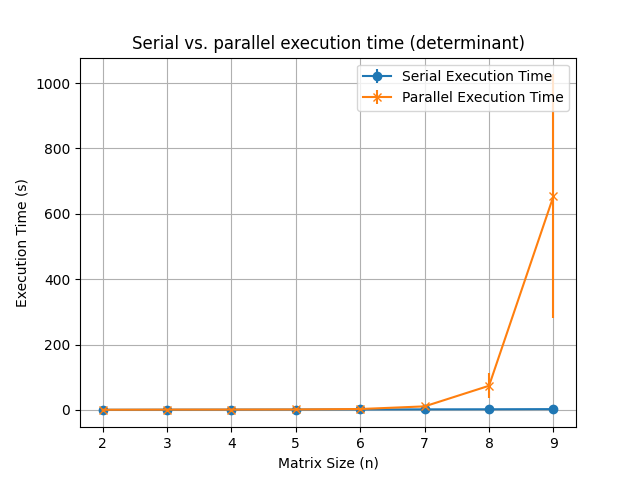
\includegraphics[width=0.8\textwidth, keepaspectratio]{img/det_2_10_3.png}
    \centering
    \label{fig:det}
    \caption{Determinant}

    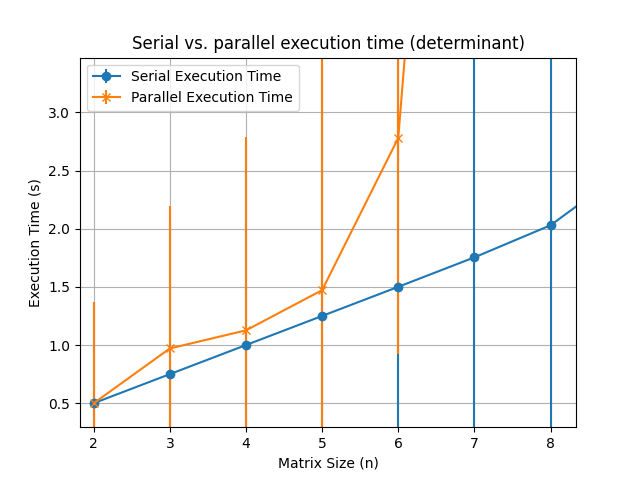
\includegraphics[width=0.8\textwidth, keepaspectratio]{img/det_2_10_3_detail.png}
    \centering
    \label{fig:det_detail}
    \caption{Detailed plot}
\end{figure}   


\subsection{Dot product}
The parallel execution times for the dot product function exhibit a similar trend compared to the determinant function. In this case, the serial execution is generally faster and increases linearly as the matrix size grows. The execution times for both serial and parallel executions are measured in microseconds ($10^{-6}$ seconds) for smaller matrices ($n \le 3$). As the matrix size increases, the performance of the parallel execution degrades, and the execution times become increasingly slower. This is in contrast to the determinant function, where the parallel execution times increased, but the performance was still somewhat decent for smaller matrices. Here, the performance gap between parallel and serial execution widens as the matrix sizes increase, suggesting that the overhead associated with parallelization becomes more pronounced for larger matrices.
\\\\
The standard deviation for serial execution times also rises with matrix size. This indicates an increased variability in execution times for larger matrices in the serial execution. In contrast, the standard deviation for parallel execution times remains relatively stable as matrix size increases, indicating more consistent results across multiple runs.
\begin{figure}[H]
    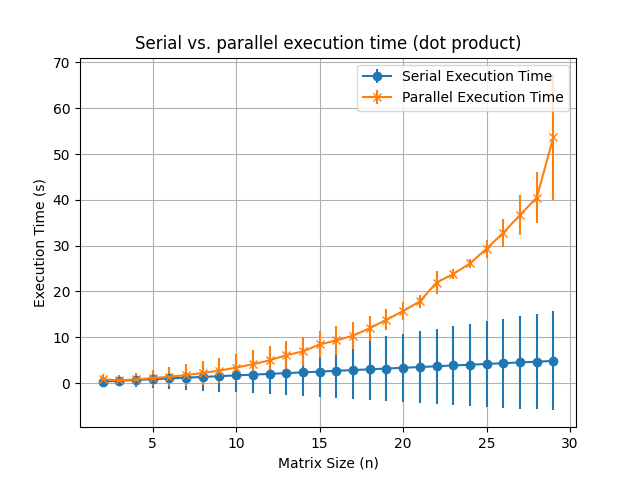
\includegraphics[width=0.8\textwidth, keepaspectratio]{img/dot_2_30_5.png}
    \centering
    \label{fig:dot}
    \caption{Dot product}

    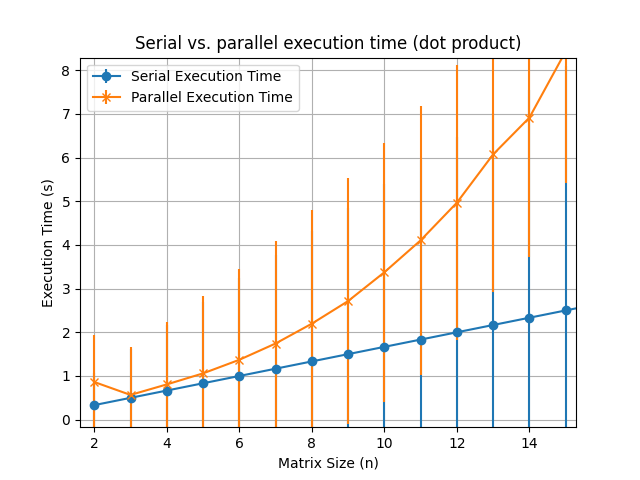
\includegraphics[width=0.8\textwidth, keepaspectratio]{img/dot_2_30_5_detail.png}
    \centering
    \label{fig:dot_detail}
    \caption{Detailed plot}
\end{figure}  

\subsection{Inverse}
In the parallel execution, the execution times for the inverse function are generally faster for smaller matrices ($n \le 3$), with execution times measured in seconds. However, for larger matrices ($n \ge 4$), the parallel execution times increase significantly, with a noticeable increase in execution times and less consistent performance. The standard deviation is also considerably higher for parallel execution in larger matrices.
\\\\
In contrast, the serial execution times for the inverse function remain relatively stable and are consistently faster than the corresponding parallel execution times for all matrix sizes. The standard deviation for serial execution is low.


\begin{figure}[H]
    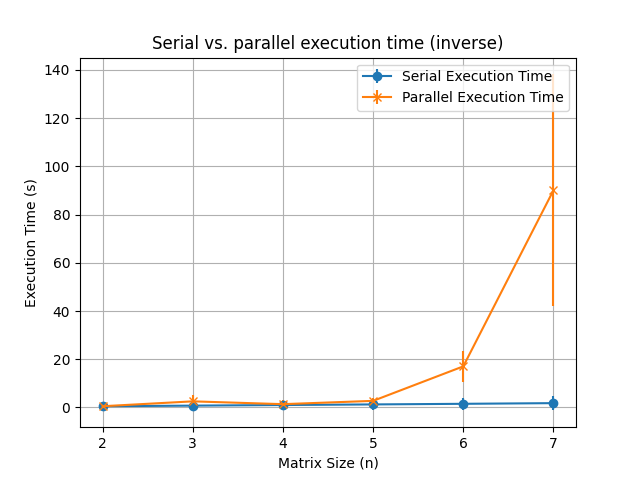
\includegraphics[width=0.8\textwidth, keepaspectratio]{img/inv_2_8_3.png}
    \centering
    \label{fig:inv}
    \caption{Inverse}

    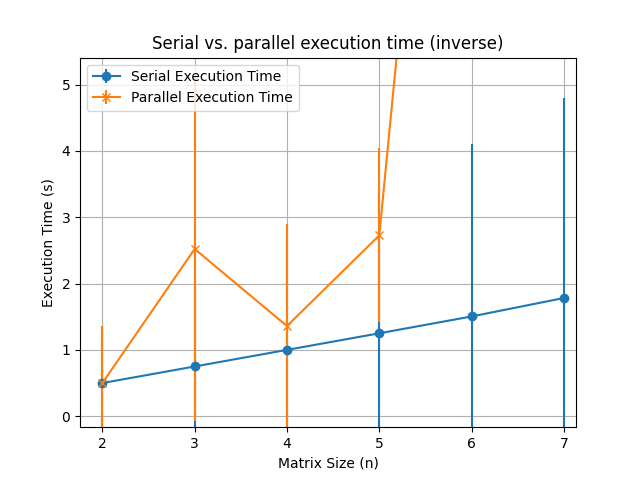
\includegraphics[width=0.8\textwidth, keepaspectratio]{img/inv_2_8_3_detail.png}
    \centering
    \label{fig:inv_detail}
    \caption{Detailed plot}
\end{figure}  

\subsection{Rank}
In the case of rank calculation, both parallel and serial show more or less the same amount of execution time, with a linear increase with the matrix size. However, the standard deviation for parallel execution increases considerably as the matrix size grows. This indicates that parallel execution becomes more variable and less consistent for larger matrices, while serial execution maintains a more stable and predictable performance.

\begin{figure}[H]
    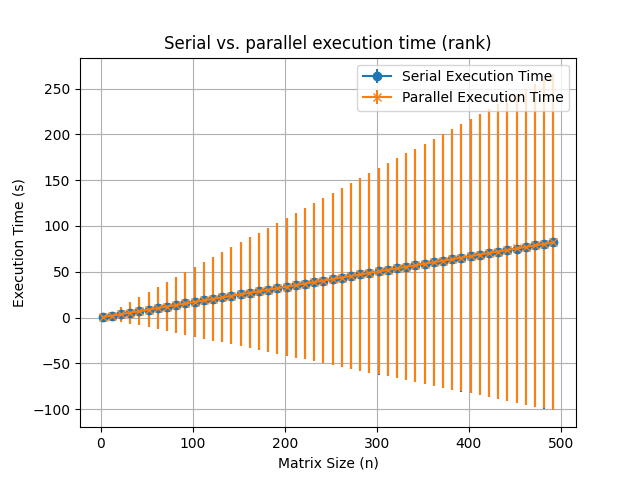
\includegraphics[width=0.8\textwidth, keepaspectratio]{img/rank_2_500_5.png}
    \centering
    \label{fig:rank}
    \caption{Rank}
\end{figure}  

\section{Conclusion}
Our investigation into the performance of distributed linear algebra operations, executed in both serial and parallel modes, has given important insights into the dynamics of distributed computing across diferent matrix sizes.

First, we observed that serial execution times, when measured in microseconds for smaller matrices ($n \le 3$), consistently outperform their parallel counterparts. However, as matrix size increases, the execution times for serial calculations grow. This trend agrees with the observation that parallel execution generally lags behind serial execution, and this performance gap widens with growing matrix sizes. This suggests that the overhead linked to parallelization can, in fact, eclipse the advantages of parallelism, especially for bigger matrices. Thus, we identified that the standard deviation of both serial and parallel execution times increase with matrix size. Altough the degree of this increase changes with the operation performed.

The standard deviation for serial execution in the dot product function also exhibits an upward trajectory with growing matrix size. In contrast, parallel execution standard deviation remains comparatively constant.

In sum, for our experiemnts, serial execution always outperforms parallel execution, with both serial execution times and standard deviations sensitive to matrix size. This reveals that the advantages of parallelization are not universally applicable, with the performance gains being countered by overhead in some scenarios.

\end{document}